
\section{Graph based reduction}
It has been shown that the graph-based representation of the atmospheric chemical network proves useful in both the visual and mathematical analysis of simulation results (\autoref{chaptervis,chaptermetric}). It therefore follows that the network representation of mechanism may also have its uses in the simplification, and thus reduction, of chemical complexity.  This section will outline the basic methods of modularity (or clustering) detection with the graph framework, the different methods in which this may be done and eventually apply it to a case example representative of the chemistry within the London environment. 









\subsection{Graph parallels. }
Although there are many graph based methods that exist within the reduction realm, most of these concentrate on the generation of skeletal methods through the building of a directed tree (subcategory of graphs from source to target) - LIST of refs and sentence of all skeletal methods. Path flux analysis (Sun et al 2010)\\

Instead we may find ourselves applying graph theory to solve other reduction methods. For instance we can trace back influence through connecting edges using dijkstras shortest path algorithm (CH2 ref) - analogous to the connectivity method, or a leave one out approach combined with pagerank to access the effects of removing a node.\\

We can use the graph structure to analyse changes of reactions or relationships between species. This can provide an alternative representation and method to access such data. Additionally we may use graph clustering techniques to locate groups of highly connected, fast reacting/strongly related species. This has applications in both understanding the data, but more importantly chemical lumping. In creating a graph from the mechanism, we not only encode information about the chemical structure, but also the rate of reaction in the graph. In grouping species by high numbers of reactions between them with fast fluxes we can take a QSSA style approach to reduction, and assume that since the rate of reaction between them is much much faster than those outside a cluster, they may be grouped together. This will be explored in PART II [ref link].








 \subsection{Types of Graph Clustering}
Unlike vector clustering algorithms (such as DBSCAN, UMAP and K-means, as discussed in SEV\autoref{veccluster}), graph clustering metrics do not rely on the spatial orientation of the data to determine groups or `clusters'. Instead these may partition the network into segments, group nodes by structual equivalence or explore the `flow' dynamics of the network. 

Algorithms such as Label Propagation \citep{labelprop} and spinglass \citep{spinglass} work by randomly assigning nodes with a property or label. This property is then transferred to its neighbours. Other algorithms such as the nested block model can decompose a graph into clusters of like properties, \citep{communitygraph}. These are often grouped in the form of topological equivalence which can be either:
\begin{itemize}
    \item[-]\textit{structual equivalence} - vertices are similar if they have like neighbours, \citep{strueq}.
    \item[-]\textit{regular eqivalence} - retrieves nodes with similar connection patterns (e.g. parent - child node hierarchicl structures), \citep{regequiv}. 
\end{itemize}
This works in a similar way to an autoencoder (ref auto \autoref{section}), where topological similarities are used to simplify (or encode) the network structure, in a way which it may be again decoded. 

Finally there exist a set of `flow' based models which use the network dynamics to determine the modularity of a network. These are discussed below. 

\subsection{Walk/Flow Based Clustering}
As temporal networks result in a change (magnitude, or type) of relationships between items. Such changes in the network dynamics are encoded within the edges of a graph. To account for this, the primary function of random walk or `flow' algorithms is to capture the the changes between the real-world systems represented by the network. 

In (SECTION SILHO) the silhouette coefficient was discussed. This compares the vector position of clusters with regards to the distance of data points between them. Translating this to the graph framework, topological (graph) clustering defines a cluster, or module, as a region with a greater inter-cluster degree or density\footnote{The number of links or edges between items in the same group.} compared to their intra-cluster density\footnote{The number of edges to other clusters}. This results in a system, that if sorted by group, has more links between elements of the same group than with those in other groups - this can be seen within the sorted adjacency matrix in (Xhaapter 1 REF). 

Since flow based methods are more interested in the network dynamics, than structure, the number of links or density is replaces with the time a random `walker' spends `trapped' between a set of nodes. A real-wold analogy would be to view the flow of water in a slowly filling river, \autoref{fig:hpp}. Here a walker (or water molecle) traverses the entirety of the river/graph network, occasionally getting trapped between a set of nodes. Here although the water is still moving, it ends up spending more time going back and fort between a set of nodes, than exploring the rest of the network. It is these regions of stalled progress that form our network clusters.  

\begin{figure}[H]
    \centering 
    \adjustbox{trim=0 2cm 0 1.4cm,clip}{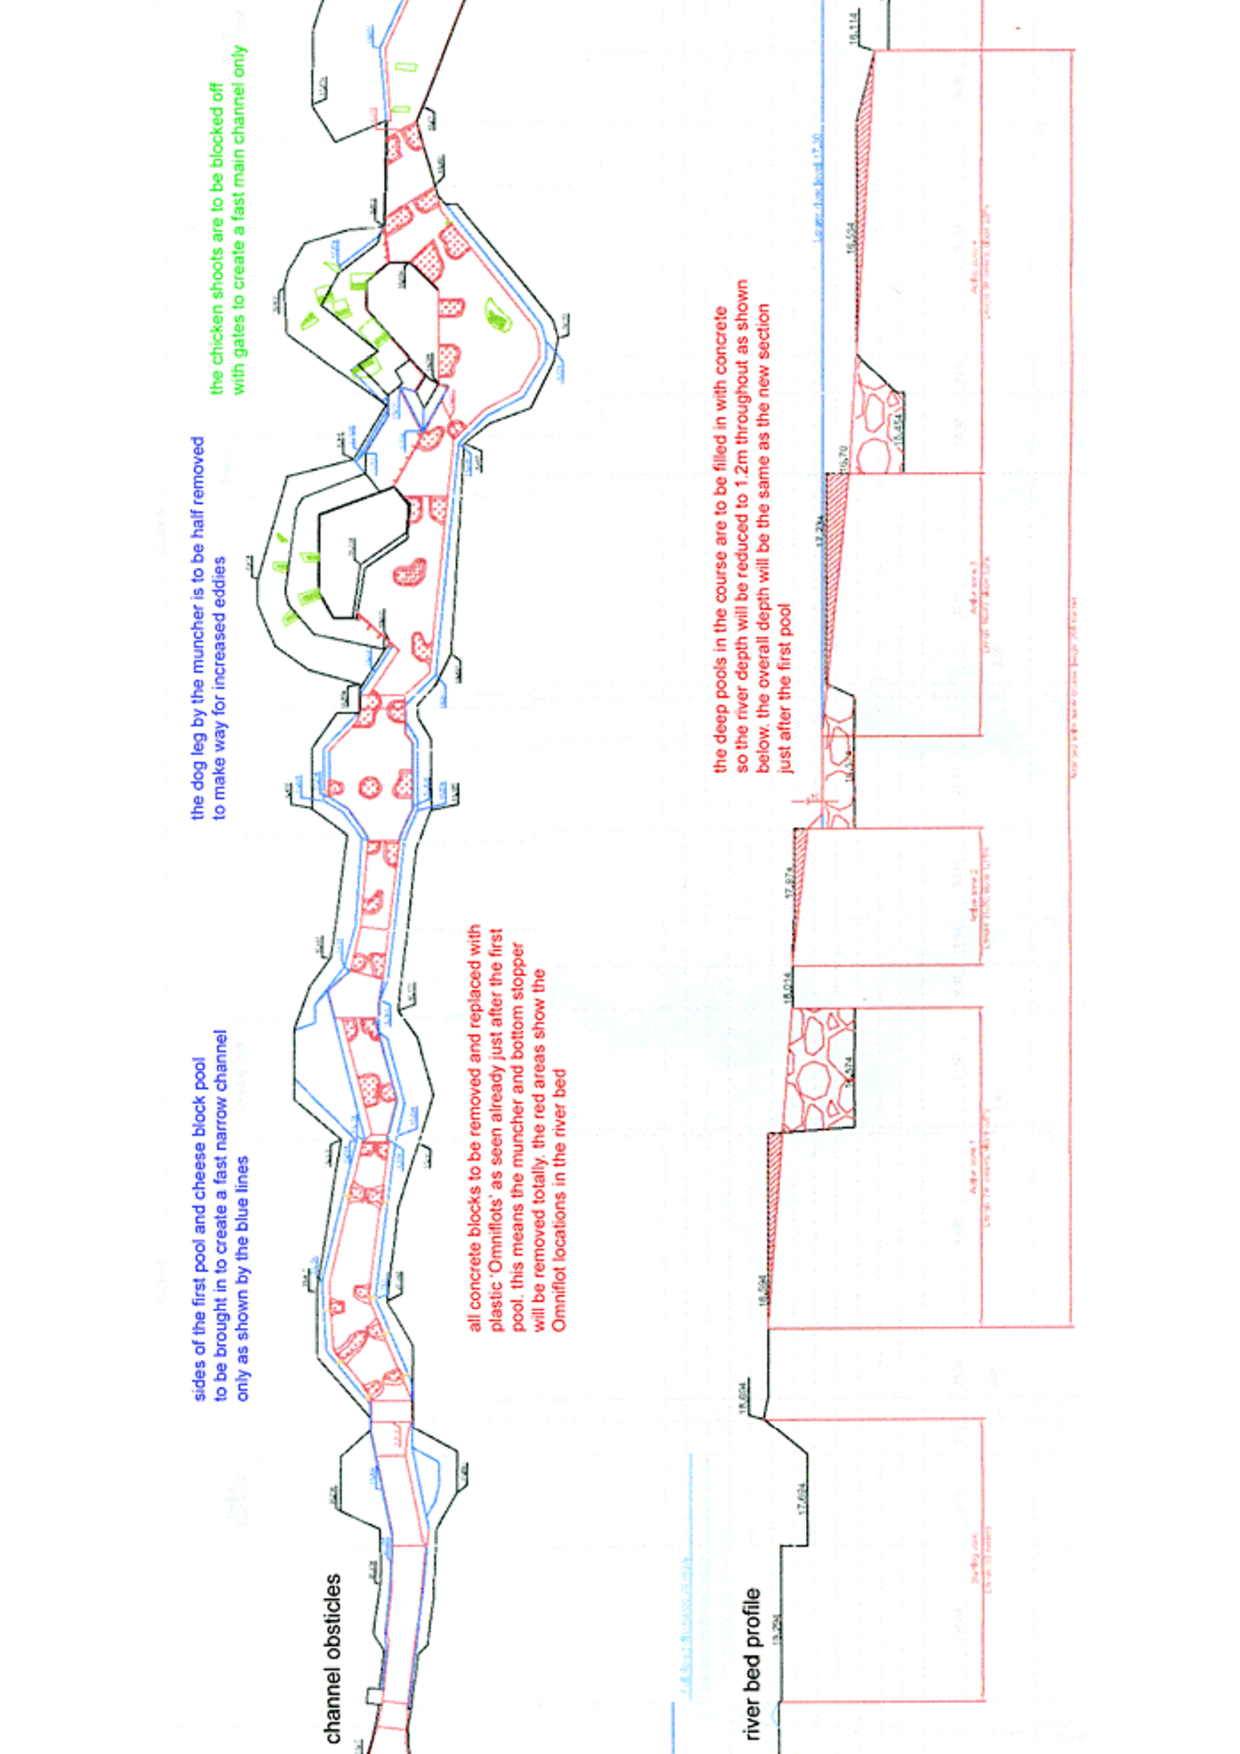
\includegraphics[height=\textwidth,angle=-90]{fig/hpp-plans.pdf}}
\caption{\textbf{The proposed plans for the change of the UK National Watersports Centre Whitewater Course (Holme Pierrepont).} Walk based clustering is analogous to the movement of a river. Clusters (or modules) are identified as areas where the `flow' becomes trapped, much like water in the pools immediately following a hydraulic jump. Source: \cite{hpp} }\label{fig:hpp}
\end{figure}

The Loudvain clustering algorithm is one of the most popular of the clustering algorithms due to its algorithmic and qualatative robustness, \citep{loudvain,loudrobust}. On the simplest level this works by maximising the modularity for each configuration. Modularity is a value between positive and negative unity which measures the density of edge between inter and intra communities and compares it to an equivalent random network.
The Loudvain is a hierarchical clustering algorith, this means that after each iteration all nodes which belong to the same cluster are consolidated to form a new `grouped' item. Inter-cluster links are converted into self-links, and intra-cluster links are updated accordingly [REF INCLUDE LAYERS OF hierarchi VCRI'

Similar to the Loudvain algorithm is the \cite{infomap}'s Infomap. Here each node within the network is assigned its own module. These are then perturbed to neighbouring nodes should such a mode lead to a decrease in the map equation (a flow-based method which operates on system dynamics rather than structure - \citep{mapeqn}). The process is repeated until no further reductions are possible.

TWO LEVEL 

MULITLEVERL

%Clustering algorithms seek to capture the intuitive notion that nodes should be connected to many nodes in the same community (intra-cluster density) but connected to few nodes in other communities (inter-cluster sparsity). We compare four clustering algorithms in this study. Each scales to networks of greater than one million nodes.

% https://www.ncbi.nlm.nih.gov/pmc/articles/PMC4938516/
% 
% The Infomap algorithm [18] is based on the principles of information theory. Infomap characterizes the problem of finding the optimal clustering of a graph as the problem of finding a description of minimum information of a random walk on the graph. The algorithm maximizes an objective function called the Minimum Description Length [19, 20], and in practice an acceptable approximation to the optimal solution can be found quickly. Previous studies have found Infomap’s performance to remain stable for networks with up to 100,000 nodes [3].

% Modularity
% The modularity of a graph compares the presence of each intra-cluster edge of the graph with the probability that that edge would exist in a random graph [23, 24]. Although modularity has been shown to have a resolution limit [25], some of the most popular clustering algorithms use it as an objective function [15, 16]. Modularity is given by Eq (1),
% 
% ∑k(ekk−a2k

% Analogously, the field-of-view limit marks an upper limit on the size of communities that Louvain and Infomap can detect [36]. Infomap’s lack of a resolution limit causes it to suffer acutely from the field-of-view limit and identify smaller clusters than Louvain identifies. In this way, the resolution limit and the field-of-view limit favor Louvain over Infomap in our experiments with large communities.

\subsection{The Infomap Clustering model}




 \twopagepicture{t}{t}{mechanism_lumping/tree.pdf}{\textbf{A radial treemap showing the hierarchical clustering of the CRI mechanism.} The simulation results used are representative of the chemistry within London at Noon localtime and generated using DSMACC and the infomap algorithm.
 }{label}{1.09}{-4}



 

 \subsubsection{Number of clusters}
 Many .... 
  resolution delimiter





















%

